\begin{boxC}
    نتایج حاصل از اجرای سه مدل یادگیری ماشین ذکرشده در تمرین به شرح زیر خواهد بود.
    همانطور که از روی متن بالای هر نتیجه مشخص است ، ما به طور کلی ۳ ویژگی بسیار معروف را برای این ۳ مدل یادگیری ماشین درنظرگرفته‌ایم.
    تعداد تکرار هر ترم ، سپس 
    \lr{TF-IDF}
    و در نهایت هم از ویژگی همسایگی بین کلمات یا همان
    \lr{Ngram}
    استفاده‌کرده‌ایم.
\end{boxC}

\begin{figure}[h]
    \centering
    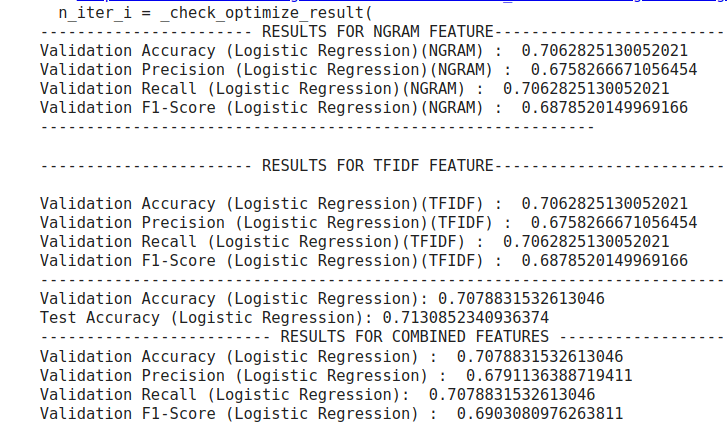
\includegraphics
    [width = 0.8\textwidth]
    {IR6/images/LR_results.png}
    \caption{\lr{Logistic Regression Results}}
    \label{fig:enter-label}
\end{figure}

\begin{boxL}
    به نظر می رسد که تفاوت قابل توجهی در عملکرد بین استفاده از ویژگی n-gram و ویژگی TF-IDF به صورت جداگانه وجود ندارد. با این حال، هنگام ترکیب هر دو ویژگی، بهبود جزئی در برخی از معیارها وجود دارد.

در اینجا چند مشاهدات بر اساس نتایج آورده شده است:

دقت: دقت برای هر دو ویژگی n-gram و ویژگی TF-IDF به صورت جداگانه در \lr{(0.7063)} یکسان است.

در صورت ترکیب، دقت کمی بهبود می یابد و به \lr{(0.7079)} می رسد. این نشان می دهد که ترکیب ویژگی ها ممکن است تأثیر مثبت کوچکی بر دقت کلی داشته باشد.

دقت، یادآوری و امتیاز F1: مقادیر دقت، فراخوانی و امتیاز F1 برای هر دو ویژگی فردی یکسان است.

با این حال، هنگام ترکیب ویژگی‌ها، بهبود جزئی در دقت \lr{(0.6791)} و امتیاز F1 \lr{(0.6903)} مشاهده می‌شود. این نشان می دهد که ترکیب ویژگی ها ممکن است به دقت بهتر و عملکرد کلی مدل کمک کند.

بر اساس این نتایج، به نظر می رسد که ترکیبی از هر دو ویژگی n-gram و TF-IDF در مقایسه با استفاده از هر ویژگی به صورت جداگانه، بهبودی حاشیه ای در عملکرد مدل ارائه می دهد. در حالی که این بهبود قابل توجه نیست،
نتیجه‌گیری کلی ما از این آزمایش این خواهد بود که :
\textbf{
اگر به دنبال پیشرفت های افزایشی در دقت و دقت کلی مدل هستید، ارزش آن را دارد که رویکرد ویژگی ترکیبی را در نظر بگیرید.
}
\end{boxL}


\begin{figure}[h]
    \centering
    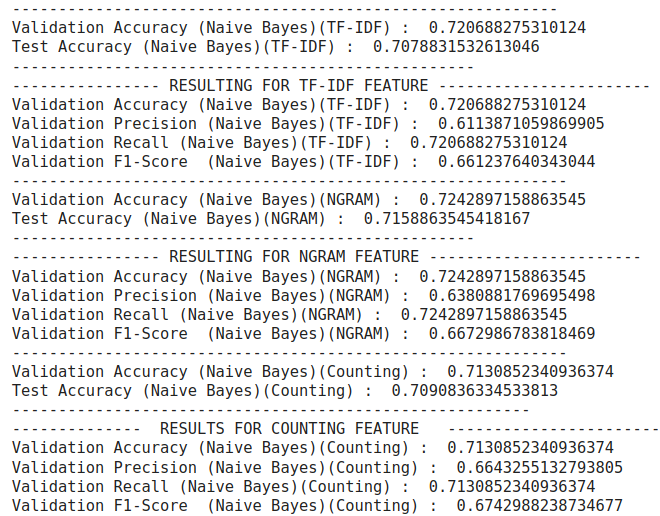
\includegraphics
    [width = 0.8\textwidth]
    {IR6/images/NB_results.png}
    \caption{\lr{Naive Bayes Results}}
    \label{fig:enter-label}
\end{figure}

\begin{boxL}

از این نتایج می توان موارد زیر را مشاهده کرد:
ویژگی NGRAM به بالاترین دقت اعتبار سنجی دست می یابد و به دنبال آن ویژگی TF-IDF قرار دارد. با این حال، هنگام در نظر گرفتن دقت تست، ویژگی TF-IDF کمی بهتر عمل می کند.
دقت، فراخوانی و امتیاز F1 الگوهای مشابهی را در بین ویژگی‌ها نشان می‌دهد، با ویژگی NGRAM به طور کلی بهتر از ویژگی‌های TF-IDF و شمارش.
شایان ذکر است که معیارهای عملکرد ممکن است بسته به مجموعه داده خاص و ماهیت مشکل طبقه بندی متفاوت باشد.
بر اساس این نتایج، به نظر می رسد که ویژگی NGRAM عملکرد کمی بهتر از خود نشان می دهد و در مقایسه با ویژگی های TF-IDF و شمارش، به دقت و امتیاز F1 بالاتری دست می یابد.
    
\end{boxL}


\begin{figure}[h]
    \centering
    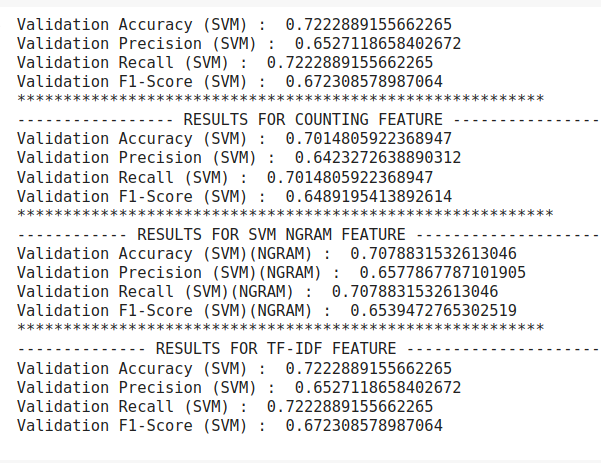
\includegraphics
    [width = 0.8\textwidth]
    {IR6/images/SVM_results.png}
    \caption{\lr{SVM Results}}
    \label{fig:enter-label}
\end{figure}

\newpage

\begin{boxL}
    از این نتایج می توان موارد زیر را مشاهده کرد:

مدل SVM با ویژگی شمارش کمترین عملکرد را در تمام معیارها، با دقت، دقت، فراخوانی و امتیاز F1 کمتر در مقایسه با سایر ویژگی ها به دست می آورد.
هر دو ویژگی NGRAM و TF-IDF عملکرد مشابهی را نشان می دهند و در مقایسه با ویژگی شمارش، به دقت، دقت، فراخوانی و امتیاز F1 بالاتری دست می یابند.
مدل SVM با ویژگی TF-IDF به بالاترین دقت اعتبارسنجی و امتیاز F1 دست می یابد، در حالی که ویژگی NGRAM دقت و یادآوری کمی بالاتری را نشان می دهد.
بر اساس این نتایج، به نظر می رسد که مدل SVM با ویژگی TF-IDF به طور کلی بهترین عملکرد را دارد و دقت و امتیاز F1 بالاتری را در مقایسه با سایر ویژگی ها نشان می دهد.
\end{boxL}

\begin{boxK}
    در نهایت می‌توان به این تبصره کلی اشاره کرد که این نتایج به دست‌آمده مربوط به داده‌های ما می‌باشد و ممکن است با توجه به تغییر بعضی هایپرپارامترها بتوان تغییرات گسترده‌تری در آن‌ها به وجود آورد.
\end{boxK}